\documentclass[10pt,a4paper]{article}
\usepackage[margin=2.2cm]{geometry}
\usepackage[T1]{fontenc}
\usepackage{lmodern,microtype,booktabs,array,tabularx,enumitem,xcolor,amsmath,amssymb}
\usepackage{tikz,pgfplots,pgfplotstable,graphicx,caption}
\usepackage[hidelinks]{hyperref}
\usepackage[most]{tcolorbox}
\usetikzlibrary{arrows.meta,positioning,shapes.symbols,calc,fit}
\pgfplotsset{compat=1.18}
\setlist{nosep,leftmargin=1.3em}
\setlength{\parindent}{0pt}\setlength{\parskip}{5pt plus 1pt}\raggedbottom
\captionsetup{font=small,labelfont=bf}

\definecolor{done}{HTML}{2E7D32}\definecolor{next}{HTML}{1565C0}
\definecolor{todo}{HTML}{9E9E9E}\definecolor{accent}{HTML}{C62828}
\definecolor{boxbg}{HTML}{F3F6FB}\definecolor{boxline}{HTML}{1565C0}
% "In plain words" boxes for readers new to machine learning
\newtcolorbox{plain}[1]{colback=boxbg,colframe=boxline,boxrule=0.5pt,arc=2pt,left=6pt,right=6pt,top=4pt,bottom=4pt,
  fonttitle=\bfseries\small,title={#1},fontupper=\small}

\newcommand{\NGames}{1'821'878}
\newcommand{\NCards}{65.6\,M}
\newcommand{\NReplayOK}{1'821'878}
\newcommand{\NPlayers}{4'608}
\newcommand{\PushRate}{62.0\,\%}
\newcommand{\DeclMean}{115.9}
\newcommand{\DeclWin}{81.0\,\%}
\newcommand{\MatchRate}{9.0\,\%}
\newcommand{\DateFrom}{2017-10-08}
\newcommand{\DateTo}{2018-04-15}
\newcommand{\JassKitRejected}{0}

\newcommand{\Cores}{14}
\newcommand{\PeakRandom}{8.9\,M}
\newcommand{\PeakHeuristic}{5.6\,M}
\newcommand{\SingleHeuristic}{956\,k}
\newcommand{\HeurDiff}{+63.9\,$\pm$\,0.1}
\newcommand{\HeurWin}{81.4\,\%}

\newcommand{\CardAcc}{79.9\,\%}
\newcommand{\CardAccChoice}{73.0\,\%}
\newcommand{\CardSamples}{123\,M}
\newcommand{\TrumpAcc}{80.1\,\%}
\newcommand{\TrumpAccFH}{81.4\,\%}

\newcommand{\StrongVsNet}{+3.3\,$\pm$\,0.6}
\newcommand{\BestAgent}{\texttt{pimc}}
\newcommand{\SearchVsNet}{+28.4\,$\pm$\,7.8}
\newcommand{\ArenaNote}{Against the human-like imitation policy, search with belief scores +28.4\,$\pm$\,7.8 points per round, the same search without belief +15.0\,$\pm$\,7.4.}


\title{\textbf{Stammtisch: Teaching a Computer to Play Schieber Jass}\\[4pt]
\large Learning from 1.8 million human games, searching over hidden cards,\\ and coaching human players}
\author{Dario Hug}
\date{Progress report, 27 September 2026}

\begin{document}
\maketitle

\begin{abstract}
\noindent
Jass is Switzerland's national card game. Its most popular variant, \emph{Schieber}, is played by two teams of two, and
every player sees only their own nine cards. This makes Jass much harder for a computer than chess: the program has
to reason about cards it cannot see, cooperate with a partner without talking, and cope with luck.
We describe \emph{Stammtisch}, a Jass program built in three layers.
(1)~A fast, exactly verified game engine that replays all \NGames{} human games of a public Swisslos dataset without a
single rule violation.
(2)~A neural network that learned to play like a typical human by studying \NCards{} human card plays; it predicts the
card a person will play \CardAcc{} of the time.
(3)~A search that imagines many possible distributions of the hidden cards, weights them by how well they explain what
the other players did, and plays each one out to see which card works best.
In matches with identical cards for both sides, the search beats the human-like network by \SearchVsNet{} points per
round. We also turned the engine into a \emph{coach}: it reviews recorded games and tells a player, with an honest error
bar, where a different card would have been better.
This report is written for readers who are new to machine learning; boxes marked \emph{``In plain words''} explain
the key ideas.
\end{abstract}

%==============================================================================
\section{Introduction}

Computers beat the best humans at chess (1997), Go (2016) and poker (2019). Card games like Jass are still an open
challenge for three reasons:
\begin{itemize}
\item \textbf{Hidden information.} You see 9 of 36 cards. The other 27 can be split among the three other players in
  about $2.3\cdot10^{12}$ ways. A good player constantly guesses who holds what.
\item \textbf{Teamwork without talking.} You win or lose with your partner, but you may not talk. Information flows
  only through which cards you play (for example, ``schmieren'': giving your partner a valuable card when their trick is safe).
\item \textbf{Luck.} A strong player with bad cards loses a single round. Measuring who is better needs many rounds and
  careful statistics.
\end{itemize}

Earlier work on Jass (Section~\ref{sec:related}) reached the level of good amateurs. Our goals are (a) a program that
beats typical human players and (b) a coach that helps a human player improve. This report makes the following
contributions:
\begin{enumerate}
\item A fast and \textbf{verified} Schieber engine with official Swisslos scoring (Weis, St\"ock, multipliers)
  (Section~\ref{sec:engine}).
\item \textbf{Imitation learning} on \NGames{} human games: neural networks that play the cards and choose trump
  like humans do (Section~\ref{sec:imitation}).
\item A \textbf{search} that samples the hidden cards, uses the networks to judge how plausible each sample is, and
  solves the end of each round exactly (Sections~\ref{sec:pimc}--\ref{sec:belief}).
\item A careful \textbf{evaluation} with duplicate deals and confidence intervals (Sections~\ref{sec:eval}--\ref{sec:results}).
\item A \textbf{coach} that reviews a player's own games (Section~\ref{sec:coach}).
\end{enumerate}

%==============================================================================
\section{Background}

\subsection{Schieber in one paragraph}
Each player gets 9 cards from a 36-card deck (four suits: Eichel, Rosen, Schilten, Schellen; ranks 6 to Ass).
The \emph{forehand} chooses the trump mode: one of the four suits, \emph{Obenabe} (no trump, high cards win) or
\emph{Undeufe} (no trump, low cards win), or they \emph{push} (``schieben'') the choice to their partner.
Then nine tricks are played: everyone must follow the suit that was led, but may always play a trump instead; the
highest card wins the trick. Among trumps the Under (Puur, 20 points) and the Nell (9, 14 points) are the strongest.
All cards together are worth 152 points, plus 5 for the last trick; a team that wins all nine tricks gets 257 (a
\emph{match}). Swisslos multiplies the points by 1 (Eichel, Rosen), 2 (Schilten, Schellen) or 3 (Obenabe, Undeufe) and
adds bonus points for card combinations (\emph{Weis}) and for holding King and Ober of trump (\emph{St\"ock}, 20 points).

\begin{figure}[h]
\centering
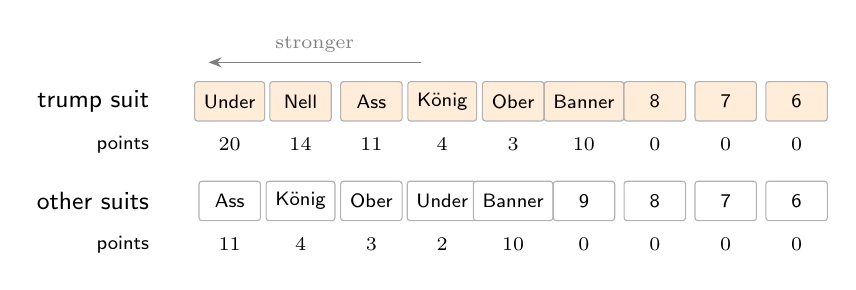
\begin{tikzpicture}[x=0.9cm,y=0.55cm,font=\small\sffamily,
  c/.style={draw=gray!60, rounded corners=1pt, minimum width=0.78cm, minimum height=0.5cm, fill=white}]
\node[anchor=east] at (0.3,0) {trump suit};
\foreach \r [count=\i] in {Under,Nell,Ass,K\"onig,Ober,Banner,8,7,6}
  \node[c, fill=orange!15] at (\i+0.3,0) {\scriptsize\r};
\foreach \p [count=\i] in {20,14,11,4,3,10,0,0,0}
  \node[font=\scriptsize] at (\i+0.3,-1) {\p};
\node[anchor=east] at (0.3,-1) {\scriptsize points};
\node[anchor=east] at (0.3,-2.3) {other suits};
\foreach \r [count=\i] in {Ass,K\"onig,Ober,Under,Banner,9,8,7,6}
  \node[c] at (\i+0.3,-2.3) {\scriptsize\r};
\foreach \p [count=\i] in {11,4,3,2,10,0,0,0,0}
  \node[font=\scriptsize] at (\i+0.3,-3.3) {\p};
\node[anchor=east] at (0.3,-3.3) {\scriptsize points};
\draw[{Stealth}-,gray] (1.0,0.9) -- node[above,font=\scriptsize]{stronger} (4.0,0.9);
\end{tikzpicture}
\caption{Card strength (left = strongest) and points. In the trump suit the Under and the 9 (Nell) jump to the top.}
\end{figure}

\subsection{How computers play games}
\begin{plain}{In plain words: the game tree and minimax}
A game can be drawn as a \emph{tree}: every position branches into the possible moves, down to the end of the game.
If you could see the whole tree, the best move is found by \emph{minimax}: assume your side picks the move that is
best for you, the opponents pick the move that is worst for you, and work backwards from the end.
\emph{Alpha-beta pruning} skips branches that cannot change the result, which makes this much faster.
\end{plain}

\begin{figure}[h]
\centering
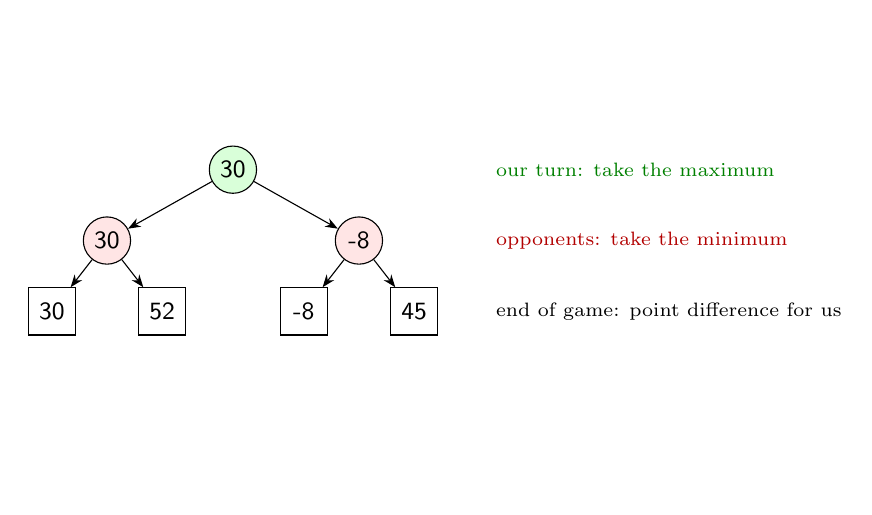
\begin{tikzpicture}[level distance=0.9cm, sibling distance=3.2cm, font=\small\sffamily,
  every node/.style={circle, draw, minimum size=6mm, inner sep=1pt},
  level 2/.style={sibling distance=1.4cm}, edge from parent/.style={draw,-{Stealth[length=1.6mm]}}]
\node[fill=green!15] {30}
  child {node[fill=red!10] {30}
    child {node[rectangle] {30}}
    child {node[rectangle] {52}}}
  child {node[fill=red!10] {-8}
    child {node[rectangle] {-8}}
    child {node[rectangle] {45}}};
\node[draw=none, anchor=west, font=\scriptsize] at (3.3,0) {\textcolor{green!50!black}{our turn: take the maximum}};
\node[draw=none, anchor=west, font=\scriptsize] at (3.3,-0.9) {\textcolor{red!70!black}{opponents: take the minimum}};
\node[draw=none, anchor=west, font=\scriptsize] at (3.3,-1.8) {end of game: point difference for us};
\end{tikzpicture}
\caption{Minimax on a tiny tree. Our left move guarantees 30 points, the right move only $-8$, so we play left.}
\end{figure}

Minimax needs to know all cards. In Jass we only know our own. The classic trick for card games is
\emph{Perfect Information Monte Carlo} (PIMC, used for Bridge~\cite{gib} and Skat~\cite{skat}): \textbf{imagine} a
possible deal of the hidden cards, solve it as if all cards were open, repeat for many imagined deals, and pick the move
that is best on average (Figure~\ref{fig:sampling}).

\begin{figure}[h]
\centering
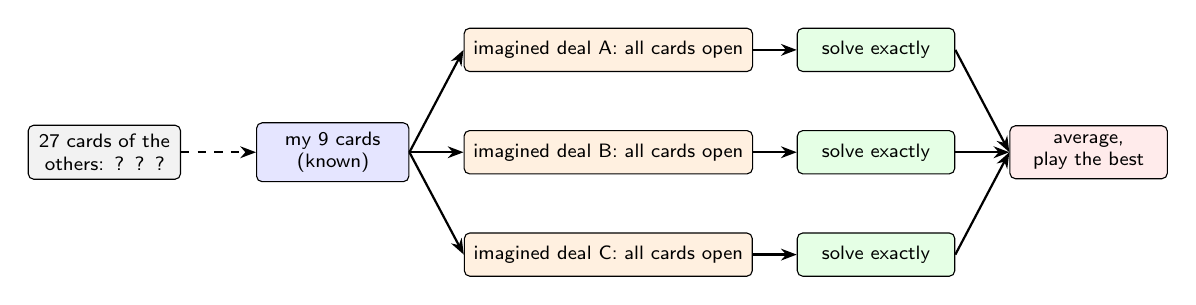
\begin{tikzpicture}[font=\scriptsize\sffamily,
  hand/.style={draw, rounded corners=2pt, minimum width=1.9cm, minimum height=0.55cm, align=center},
  arr/.style={-{Stealth[length=2mm]}, thick}]
\node[hand, fill=blue!10, text width=1.7cm] (me) at (0,0) {my 9 cards\\(known)};
\node[hand, fill=gray!10, text width=1.7cm] (hid) at (-2.9,0) {27 cards of the others: ? ? ?};
\draw[arr, dashed] (hid) -- (me);
\foreach \w/\y in {A/1.3, B/0, C/-1.3} {
  \node[hand, fill=orange!12, minimum width=2.6cm] (w\w) at (3.5,\y) {imagined deal \w: all cards open};
  \draw[arr] (me.east) -- (w\w.west);
  \node[hand, fill=green!10, minimum width=2.0cm] (s\w) at (6.9,\y) {solve exactly};
  \draw[arr] (w\w) -- (s\w);
}
\node[hand, fill=red!8, minimum width=2.0cm] (avg) at (9.6,0) {average,\\ play the best};
\foreach \w in {A,B,C} \draw[arr] (s\w.east) -- (avg.west);
\end{tikzpicture}
\caption{The idea behind PIMC: fill in the unknown cards in many plausible ways, solve each imagined deal,
and average the results.}
\label{fig:sampling}
\end{figure}

\subsection{Machine learning in a nutshell}
\begin{plain}{In plain words: what a neural network is and how it learns}
A \emph{neural network} is a function with many adjustable numbers (``weights''). It takes a list of numbers as input
(here: which cards I hold, which cards were played, what trump is) and outputs a score for every possible card.
\emph{Training} means showing it millions of examples (``in this situation, the human played the Rosen Ass'') and
nudging the weights a tiny bit after each example so that the correct answer gets a higher score next time.
To check that the network learned something general instead of memorizing, we test it on \emph{validation} games it
never saw during training.
\end{plain}

\begin{figure}[h]
\centering
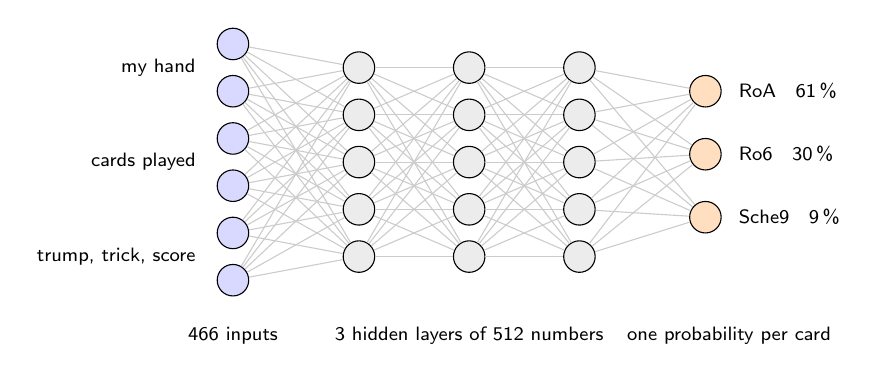
\begin{tikzpicture}[font=\scriptsize\sffamily, neuron/.style={circle, draw, minimum size=4mm, inner sep=0}]
\foreach \y [count=\i] in {1.6,1.0,0.4,-0.2,-0.8,-1.4} \node[neuron, fill=blue!15] (i\i) at (0,\y) {};
\node[anchor=east] at (-0.35,1.3) {my hand};
\node[anchor=east] at (-0.35,0.1) {cards played};
\node[anchor=east] at (-0.35,-1.1) {trump, trick, score};
\foreach \L/\x in {a/1.6,b/3.0,c/4.4}
  \foreach \y [count=\i] in {1.3,0.7,0.1,-0.5,-1.1} \node[neuron, fill=gray!15] (\L\i) at (\x,\y) {};
\foreach \y [count=\i] in {1.0,0.2,-0.6} \node[neuron, fill=orange!25] (o\i) at (6.0,\y) {};
\node[anchor=west] at (6.3,1.0) {RoA \; 61\,\%};
\node[anchor=west] at (6.3,0.2) {Ro6 \; 30\,\%};
\node[anchor=west] at (6.3,-0.6) {Sche9 \; 9\,\%};
\foreach \i in {1,...,6} \foreach \j in {1,...,5} \draw[gray!40] (i\i) -- (a\j);
\foreach \i in {1,...,5} \foreach \j in {1,...,5} {\draw[gray!40] (a\i) -- (b\j); \draw[gray!40] (b\i) -- (c\j);}
\foreach \i in {1,...,5} \foreach \j in {1,...,3} \draw[gray!40] (c\i) -- (o\j);
\node at (0,-2.1) {466 inputs}; \node at (3.0,-2.1) {3 hidden layers of 512 numbers}; \node at (6.3,-2.1) {one probability per card};
\end{tikzpicture}
\caption{The card network. It reads the situation as 466 numbers and outputs a probability for each legal card.
The real network is much larger than drawn.}
\label{fig:net}
\end{figure}

\subsection{Related work}\label{sec:related}
Jass has been studied mainly at Swiss universities. The Lucerne University of Applied Sciences (HSLU) teaches a
course \emph{Deep Learning for Games} built around Jass and provides the \texttt{jass-kit} software~\cite{jasskit} and
the Swisslos dataset we use. A survey from the University of Fribourg~\cite{survey} compares approaches, and theses at
the University of Bern tried AlphaZero-style learning and game-theoretic methods; the best programs reached the level of
strong amateurs. Our approach combines ideas from Bridge (PIMC~\cite{gib,long}), Skat (learning about the opponents'
cards from their play~\cite{skat}) and AlphaZero-style self-improvement~\cite{alphazero}.

%==============================================================================
\section{Data}\label{sec:data}
The dataset contains \NGames{} Schieber rounds played online at Swisslos between \DateFrom{} and \DateTo{} by
\NPlayers{} registered players. Each round lists all nine tricks, so we can reconstruct all four hands. This gives
\NCards{} card decisions and about 3~million trump decisions, each with the correct ``answer'' (what the human did).
We keep the most recent 5\,\% of games (by date) apart as validation data.

\begin{figure}[h]
\centering
\begin{tikzpicture}
\begin{axis}[width=0.48\textwidth, height=4.6cm, ybar stacked, bar width=13pt, ymin=0,
  ylabel={\% of games}, xtick=data, symbolic x coords={0,1,2,3,4,5},
  xticklabels={Eichel {\scriptsize$\times$1},Rosen {\scriptsize$\times$1},Schilten {\scriptsize$\times$2},Schellen {\scriptsize$\times$2},Obe {\scriptsize$\times$3},Une {\scriptsize$\times$3}},
  x tick label style={font=\scriptsize, rotate=30, anchor=east},
  legend style={font=\scriptsize, at={(0.02,0.98)}, anchor=north west}, title={\small Which trump do humans choose?}]
\addplot[fill=blue!55, draw=none] table[x=idx, y=share_direct, col sep=comma] {data/trump.csv};
\addplot[fill=orange!70, draw=none] table[x=idx, y=share_pushed, col sep=comma] {data/trump.csv};
\legend{forehand, after push}
\end{axis}
\end{tikzpicture}\hfill
\begin{tikzpicture}
\begin{axis}[width=0.48\textwidth, height=4.6cm, ybar, bar width=4pt, ymin=0, xmin=0, xmax=265,
  xlabel={points of the team that chose trump}, ylabel={\% of games}, title={\small How well does the declaring team do?},
  extra x ticks={78.5}, extra x tick labels={}, extra x tick style={grid=major, grid style={dashed, accent}}]
\addplot[fill=blue!55, draw=none] table[x=bin, y=share, col sep=comma] {data/decl_points.csv};
\end{axis}
\end{tikzpicture}
\caption{Left: players push in \PushRate{} of rounds and prefer the high-multiplier modes when they choose directly.
Right: the team that chose trump wins \DeclWin{} of rounds (dashed line: half of 157); \MatchRate{} of rounds are matches.}
\end{figure}

%==============================================================================
\section{Method}\label{sec:method}

\begin{figure}[h]
\centering
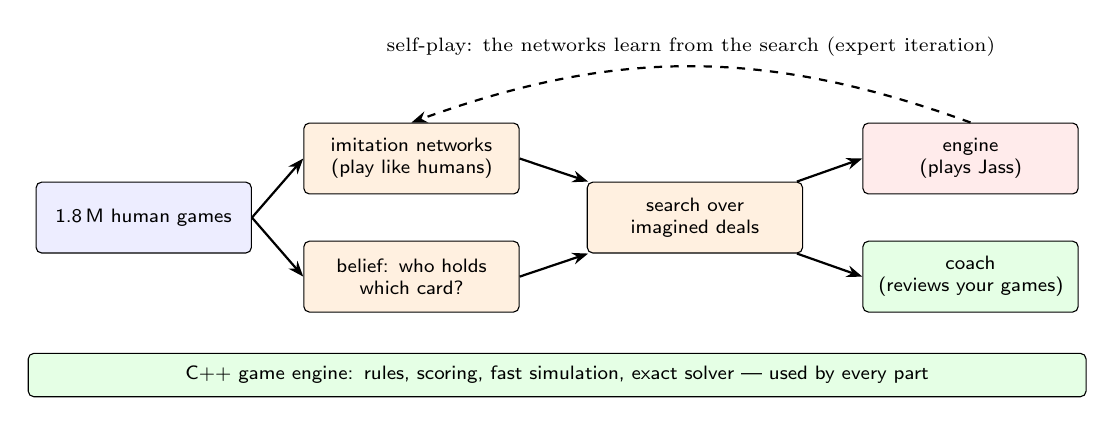
\begin{tikzpicture}[
  box/.style={draw, rounded corners=2pt, minimum height=0.9cm, text width=2.5cm, align=center, font=\scriptsize\sffamily},
  data/.style={box, fill=blue!7}, model/.style={box, fill=orange!12},
  arr/.style={-{Stealth[length=2mm]}, thick}]
\node[data]  (logs)   at (0,-0.75)  {1.8\,M human games};
\node[model] (sl)     at (3.4,0)    {imitation networks\\(play like humans)};
\node[model] (belief) at (3.4,-1.5) {belief: who holds\\which card?};
\node[model] (search) at (7.0,-0.75) {search over\\imagined deals};
\node[box, fill=red!8] (out) at (10.5,0) {engine\\(plays Jass)};
\node[box, fill=green!10] (coach) at (10.5,-1.5) {coach\\(reviews your games)};
\draw[arr] (logs.east) -- (sl.west); \draw[arr] (logs.east) -- (belief.west);
\draw[arr] (sl.east) -- (search); \draw[arr] (belief.east) -- (search);
\draw[arr] (search) -- (out.west); \draw[arr] (search) -- (coach.west);
\draw[arr, dashed] (out.north) to[bend right=20] node[above, font=\scriptsize] {self-play: the networks learn from the search (expert iteration)} (sl.north);
\node[box, fill=green!10, text width=13.2cm, minimum height=0.55cm] at (5.25,-2.75)
  {C++ game engine: rules, scoring, fast simulation, exact solver --- used by every part};
\end{tikzpicture}
\caption{Overview. Human games teach the networks; the networks guide the search; the search plays, coaches, and
produces new training data for the networks.}
\end{figure}

\subsection{Game engine and simulator}\label{sec:engine}
The engine stores a hand as a 64-bit number in which bit $i$ says whether card $i$ is present. Checking which cards may
legally be played then takes a handful of processor instructions. On a laptop (\Cores{} threads) the simulator plays
\PeakRandom{} rounds per second. A live dashboard shows throughput, results, CPU load and temperature while it runs.

\textbf{Verification.} Bugs in the rules would silently poison everything built on top. We therefore replayed every
one of the \NGames{} human games: all \NCards{} card plays are legal and every trick winner and score matches the log.
We also compared our rules with HSLU's \texttt{jass-kit} on 119\,073 random positions. The only disagreements (0.15\,\%)
turned out to be a bug in \texttt{jass-kit}, which in rare cases allows ``under-trumping''.

\subsection{Exact solver for open cards}\label{sec:dd}
If all cards were visible, the best play could be computed exactly with minimax and alpha-beta pruning. In card games
this is called a \emph{double-dummy} solver. Three standard tricks make ours fast: it remembers positions it has already
solved (a \emph{transposition table}), treats cards that are interchangeable (e.g.\ the 7 and the 6 when nothing lies
between them) as one, and narrows in on the exact score with a sequence of yes/no questions (\emph{MTD(f)}~\cite{mtdf}).
It agrees with a brute-force search on 2\,560 random endgames. Its cost grows about tenfold per extra trick
(Figure~\ref{fig:speed}), so we use it for the last $k=5$ tricks only.

\subsection{Imitation learning: playing like a human}\label{sec:imitation}
The \emph{card network} (Figure~\ref{fig:net}) receives what the player can see, encoded as 466 zeros and ones:
own hand, cards played by each player, the cards in the current trick, trump, who chose trump, which suits a player
has shown to be out of, and the score. It outputs a probability for each of the 36 cards; illegal cards are masked out.
It was trained on \CardSamples{} examples, about 40 minutes on the laptop's processor. A second, smaller
\emph{trump network} looks at the 9 cards of a hand and predicts the trump choice (or push).

\begin{plain}{In plain words: why imitate humans at all?}
Imitation gives us three things at once: a decent player without any hand-written rules; a \emph{model of human
behaviour} (``how likely would a person play this card with that hand?''), which we need for the belief in
Section~\ref{sec:belief}; and a realistic \emph{sparring partner} to measure our engine against.
\end{plain}

\subsection{Search over imagined deals}\label{sec:pimc}
To choose a card, the engine repeats $n=32$ times: (1) imagine a deal of the hidden cards that agrees with everything the
player has seen (for example, a player who did not follow suit has no card of that suit left), (2) for each legal
card, play the rest of the round: the human-like network plays for everybody until 5 tricks are left, then the exact
solver finishes the round, (3) note the resulting point difference. The card with the best average wins.
The trump choice is made by the trump network: a search over all six modes was not better (Section~\ref{sec:results}).

\subsection{Belief: learning from the other players' behaviour}\label{sec:belief}
Uniformly imagined deals ignore valuable hints. If your opponent chose Rosen as trump, they probably hold the Rosen
Under; if your partner pushed, their hand is probably weak. We use the networks to ask, for each imagined deal:
\emph{how likely would the other players have made exactly the choices we saw, if this were the true deal?} Deals that
explain the observed play well get a higher weight (this is Bayes' rule). In practice we imagine $4n$ deals, weight
them by this likelihood raised to the power $b=0.5$ (a softening that keeps the method robust when people play
differently from the model), and keep $n$ of them in proportion to their weights.

\begin{plain}{In plain words: a small example of the belief}
Imagine two possible worlds. In world A your left opponent holds the Rosen Under, in world B they do not. They chose
Rosen as trump. Suppose the trump network says: with the Under, a human picks Rosen 70\,\% of the time; without it,
only 5\,\%. Then world A becomes 14 times more likely than before, and the search spends most of its effort on deals
like A.
\end{plain}

\subsection{Expert iteration: learning from the search}\label{sec:expit}
The search plays better than the network it uses. So we let the search play 8\,000 rounds against itself (one hour on
the laptop) and trained a copy of the network on the search's 288\,000 decisions, mixed with 25\,\% human data so it
does not forget what it knew. Its agreement with the search on unseen positions rose from 54.7\,\% to 61.4\,\% of the
real choices. This is the idea behind AlphaZero~\cite{alphazero}: the search improves the network, and a better network
improves the search. We call the result \texttt{net:strong}.

\begin{figure}[h]
\centering
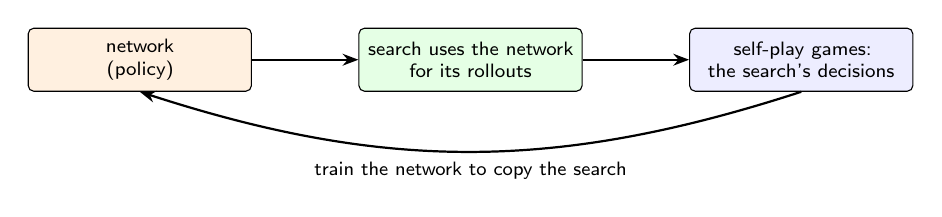
\begin{tikzpicture}[font=\scriptsize\sffamily, box/.style={draw, rounded corners=2pt, minimum height=0.8cm, text width=2.6cm, align=center},
  arr/.style={-{Stealth[length=2mm]}, thick}]
\node[box, fill=orange!12] (net) at (0,0) {network\\(policy)};
\node[box, fill=green!10] (search) at (4.2,0) {search uses the network\\for its rollouts};
\node[box, fill=blue!7] (games) at (8.4,0) {self-play games:\\the search's decisions};
\draw[arr] (net) -- (search); \draw[arr] (search) -- (games);
\draw[arr] (games.south) to[bend left=18] node[below] {train the network to copy the search} (net.south);
\end{tikzpicture}
\caption{Expert iteration: a loop in which the network and the search improve each other. We have run one round.}
\end{figure}

\subsection{The coach}\label{sec:coach}
A recorded game is typed in a simple text format (players, dealer, trump, and the tricks, with German or French card
names). For every decision the coach runs the same search \emph{from that player's point of view}, using only what they
could see, and reports how many points each alternative card was expected to gain or lose. Because the search is based
on random samples, every number comes with a standard error; only losses clearly larger than this noise are called
mistakes. The coach also gives a one-line reason taken from the actual trick (e.g.\ ``schmieren: RoB gives your team 10
more points'') and, in the last tricks, the exact best card with all hands open. The same evaluation is available live
(``which card should I play now?'') and while playing against the engine.

%==============================================================================
\section{How we measure strength}\label{sec:eval}
\begin{plain}{In plain words: fair comparisons in a game of luck}
\textbf{Duplicate deals.} Every deal is played twice: once agent A holds the North/South cards, once the East/West
cards. Good or bad cards then cancel out, and mostly skill remains.\\
\textbf{Confidence interval.} We report results like ``$+28 \pm 8$ points per round'': the true advantage lies within
this range with 95\,\% probability. If the range does not include 0, the difference is \emph{significant}.\\
\textbf{Elo.} Like in chess, a rating derived from how often one agent wins rounds against another; 100 points more
means winning about 64\,\% of rounds against that opponent.
\end{plain}

We compare these agents: \texttt{random} (random legal cards), \texttt{heuristic} (hand-written rules, e.g.\ lead your
highest card, give points to a winning partner), \texttt{net} (imitation of humans), \texttt{net:strong} (after expert
iteration), \texttt{pimc} (search with belief), and variants of the search. All numbers are in \emph{slate points}
(with Swisslos multipliers, Weis and St\"ock), per round.

%==============================================================================
\section{Results}\label{sec:results}

\subsection{Speed}
\begin{figure}[h]
\centering
\begin{tikzpicture}
\begin{axis}[width=0.48\textwidth, height=4.8cm, xlabel={threads}, ylabel={million rounds / s}, ymin=0,
  legend style={font=\scriptsize, at={(0.02,0.98)}, anchor=north west}, grid=major, grid style={gray!20},
  title={\small Simulator throughput (laptop)}]
\addplot+[mark=*, thick] table[x=threads, y expr=\thisrow{random}/1e6, col sep=comma] {data/scaling.csv};
\addplot+[mark=square*, thick] table[x=threads, y expr=\thisrow{heuristic}/1e6, col sep=comma] {data/scaling.csv};
\legend{random agents, heuristic agents}
\end{axis}
\end{tikzpicture}\hfill
\begin{tikzpicture}
\begin{semilogyaxis}[width=0.48\textwidth, height=4.8cm, xlabel={tricks left to play}, ylabel={ms per exact solve},
  grid=major, grid style={gray!20}, title={\small Exact solver: cost grows fast}]
\addplot+[mark=*, thick] table[x=left, y=mean_ms, col sep=comma] {data/dd_timing.csv};
\end{semilogyaxis}
\end{tikzpicture}
\caption{Left: the simulator scales over the laptop's cores. Right: solving a position exactly takes about a
millisecond with 5 tricks left but seconds with 8, which is why the search solves only the last 5 tricks exactly.}
\label{fig:speed}
\end{figure}

\subsection{How well does the network imitate humans?}
\begin{minipage}[t]{0.5\textwidth}
\vspace{0pt}
\begin{tikzpicture}
\begin{axis}[width=\textwidth, height=4.8cm, xlabel={training examples seen (millions)}, ylabel={correct predictions (\%)},
  legend style={font=\scriptsize, at={(0.98,0.03)}, anchor=south east}, grid=major, grid style={gray!20},
  title={\small Learning curve on unseen games}]
\addplot+[mark=none, thick] table[x=samples_m, y=val_acc, col sep=comma] {data/train_card.csv};
\addplot+[mark=none, thick] table[x=samples_m, y=val_acc_nonforced, col sep=comma] {data/train_card.csv};
\legend{all decisions, only real choices}
\end{axis}
\end{tikzpicture}
\end{minipage}\hfill
\begin{minipage}[t]{0.46\textwidth}
\vspace{4pt}
The network predicts the human's card in \CardAcc{} of validation decisions and in \CardAccChoice{} of the decisions
where more than one card was legal. The trump network matches \TrumpAcc{} of human trump calls.
The curve flattens after about 60~million examples: more of the same data would not help much.

A perfect score is impossible: two humans in the same situation often play differently, and many decisions are close.
\end{minipage}

\subsection{Who plays best?}
\begin{minipage}[t]{0.33\textwidth}
\vspace{0pt}\small
\pgfplotstabletypeset[col sep=semicolon, string type,
  columns/rank/.style={column name=\#},
  columns/agent/.style={column name=agent, column type=l, postproc cell content/.append style={/pgfplots/table/@cell content/.add={\ttfamily\scriptsize}{}}},
  columns/elo/.style={column name=Elo, column type=r},
  every head row/.style={before row=\toprule, after row=\midrule}, every last row/.style={after row=\bottomrule}]
  {data/leaderboard.csv}
\end{minipage}\hfill
\begin{minipage}[t]{0.64\textwidth}
\vspace{0pt}\scriptsize
\pgfplotstabletypeset[col sep=semicolon, string type,
  columns={a,b,deals,diff,ci95},
  columns/a/.style={column name=A, column type=l, postproc cell content/.append style={/pgfplots/table/@cell content/.add={\ttfamily}{}}},
  columns/b/.style={column name=B, column type=l, postproc cell content/.append style={/pgfplots/table/@cell content/.add={\ttfamily}{}}},
  columns/deals/.style={column name=deals, column type=r},
  columns/diff/.style={column name={A$-$B per round}, column type=r},
  columns/ci95/.style={column name=$\pm$, column type=r},
  every head row/.style={before row=\toprule, after row=\midrule}, every last row/.style={after row=\bottomrule}]
  {data/matches.csv}
\end{minipage}

\medskip
The main findings:
\begin{itemize}
\item \textbf{Learning beats hand-written rules.} The imitation network beats the heuristic by almost 100 points per round.
\item \textbf{Search beats imitation.} The search agent \texttt{pimc} beats the human-like network by \SearchVsNet{}
  points per round. This is our best estimate of its advantage over a typical online player, with the caveat that the
  network is only a stand-in for real humans.
\item \textbf{The belief matters.} \ArenaNote
\item \textbf{Expert iteration works, a little.} After one round, \texttt{net:strong} beats the human imitation by
  \StrongVsNet{} points per round (significant over 40\,000 deals). Using it inside the search did not yet make a
  measurable difference.
\end{itemize}

\textbf{What did not help.} Each variant played 600 duplicate deals against the earlier default search
(32 samples, trump by searching 16 deals per mode, exact for 5 tricks, belief 0.5); positive = variant better:

\begin{center}\small
\pgfplotstabletypeset[col sep=semicolon, string type,
  columns={variant,change,diff,ci95},
  columns/variant/.style={column name=variant, column type=l, postproc cell content/.append style={/pgfplots/table/@cell content/.add={\ttfamily}{}}},
  columns/change/.style={column name=change, column type=l},
  columns/diff/.style={column name={points / round}, column type=r},
  columns/ci95/.style={column name=$\pm$, column type=r},
  every head row/.style={before row=\toprule, after row=\midrule}, every last row/.style={after row=\bottomrule}]
  {data/tuning.csv}
\end{center}
None of these differences is significant. Interestingly, choosing trump the way humans do is as good as searching over
all six modes, and much faster, so it became the default.

\subsection{The coach in action}
Figure~\ref{fig:coach} shows a review of an example round. Each card played by the reviewed team is marked green
(good), yellow/orange/red (increasingly costly) or grey (difference within the sampling noise). As a sanity check, the
coach judged random play worst, the heuristic better and the human-like network best, as it should.

\begin{figure}[h]
\centering
\IfFileExists{data/review.png}{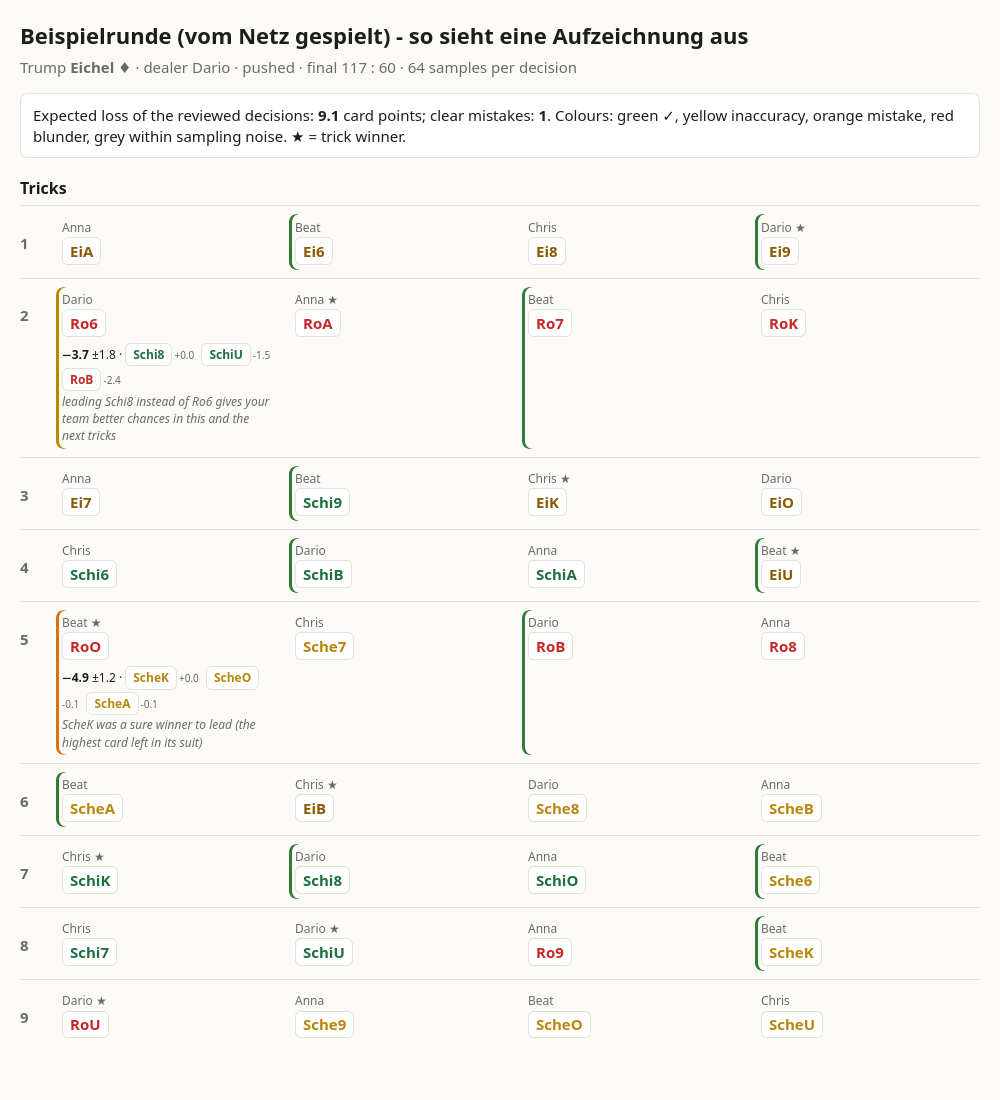
\includegraphics[width=0.66\textwidth,trim=0 330 0 0,clip]{data/review.png}}{}
\caption{HTML review of a round. In trick 2 the coach suggests leading a different card than Ro6; the difference is
within the sampling noise, so it is shown in grey rather than as a mistake.}
\label{fig:coach}
\end{figure}

%==============================================================================
\section{Discussion and limitations}
\begin{itemize}
\item \textbf{Humans are not networks.} Our strongest evidence compares against a network that imitates average
  Swisslos players. Real people plan ahead, use conventions with their partner and adapt. The next step is to play
  against real people, for example in the HSLU tournament system, for which we already built an adapter.
\item \textbf{Imagining is not knowing.} PIMC solves each imagined deal as if everyone could see all cards. It can
  therefore overrate plays that only work with perfect knowledge (``strategy fusion''~\cite{long}). The rollouts with
  the human-like network soften this, but do not remove it.
\item \textbf{Small experiments.} Many of our comparisons used 400--600 deals, which can only detect differences of
  about 8 points per round. Smaller improvements need more compute.
\item \textbf{Data licence.} The Swisslos data comes from public course material; we have asked HSLU for permission to
  use it and do not publish the data or the trained networks until then.
\end{itemize}

%==============================================================================
\section{Conclusion and next steps}
With a verified engine, imitation of 1.8~million human games, and a search that reasons about hidden cards and about
what the other players' choices reveal, Stammtisch beats a human-like opponent by \SearchVsNet{} points per round, and
it can show a player where their own games went wrong. Next we plan to (1) run more rounds of expert iteration with a
larger compute budget, (2) replace the rollouts by a network that directly predicts the outcome of a position (a
\emph{value network}), (3) speed up the exact solver, and (4) test the engine and the coach against real players.

\begin{plain}{Glossary}
\textbf{Validation data:} examples held back from training to test the network honestly. \enspace
\textbf{Policy:} a rule (here: a network) that picks a move. \enspace
\textbf{Rollout:} playing a round to the end with a policy to see what happens. \enspace
\textbf{Double dummy:} solving a deal with all cards open. \enspace
\textbf{PIMC:} imagine the hidden cards, solve each imagined deal, average. \enspace
\textbf{Belief:} how likely each distribution of the hidden cards is, given what we saw. \enspace
\textbf{Expert iteration:} training a network to copy a stronger search. \enspace
\textbf{Duplicate deals:} playing each deal twice with swapped seats to cancel luck. \enspace
\textbf{Significant:} unlikely to be a coincidence (here: the 95\,\% range excludes zero).
\end{plain}

\begin{thebibliography}{9}\small\setlength{\itemsep}{1pt}\setlength{\parskip}{0pt}
\bibitem{survey} J.~Niklaus, M.~Alberti, V.~Pondenkandath, R.~Ingold, M.~Liwicki. \emph{Survey of Artificial
  Intelligence for Card Games and Its Application to the Swiss Game Jass.} Swiss Conference on Data Science, 2019.
\bibitem{gib} M.~L.~Ginsberg. \emph{GIB: Imperfect information in a computationally challenging game.} Journal of
  Artificial Intelligence Research, 2001.
\bibitem{long} J.~Long, N.~Sturtevant, M.~Buro, T.~Furtak. \emph{Understanding the success of perfect information
  Monte Carlo sampling in game tree search.} AAAI, 2010.
\bibitem{skat} M.~Buro, J.~Long, T.~Furtak, N.~Sturtevant. \emph{Improving state evaluation, inference, and search in
  trick-based card games.} IJCAI, 2009.
\bibitem{mtdf} A.~Plaat, J.~Schaeffer, W.~Pijls, A.~de~Bruin. \emph{Best-first fixed-depth minimax algorithms.}
  Artificial Intelligence, 1996.
\bibitem{alphazero} D.~Silver et al. \emph{A general reinforcement learning algorithm that masters chess, shogi, and
  Go through self-play.} Science, 2018.
\bibitem{jasskit} HSLU, \emph{jass-kit-py}, \url{https://github.com/thomas-koller/jass-kit-py};
  Swisslos Schieber rules, \url{https://www.swisslos.ch/de/jass/informationen/jass-regeln/schieber-jass.html}.
\end{thebibliography}
\end{document}
